\begin{table}[h!]
    \centering
    \begin{tabular}{lcccc}
        \hline
        \textbf{Class} & \textbf{Precision} & \textbf{Recall} & \textbf{F1-Score} & \textbf{Support} \\
        \hline
        0.0 & 0.77 & 0.68 & 0.72 & 10604 \\
        1.0 & 0.71 & 0.79 & 0.75 & 10604 \\
        \hline
        \textbf{Accuracy} & \multicolumn{3}{c}{0.74} & 21208 \\
        \textbf{Macro Avg} & 0.74 & 0.74 & 0.74 & 21208 \\
        \textbf{Weighted Avg} & 0.74 & 0.74 & 0.74 & 21208 \\
        \hline
    \end{tabular}
    \caption{Classification Report for Autoencoder}
    \label{tab:autoencoder_classification_report}
\end{table}

\vspace{0.5cm}
\begin{center}
    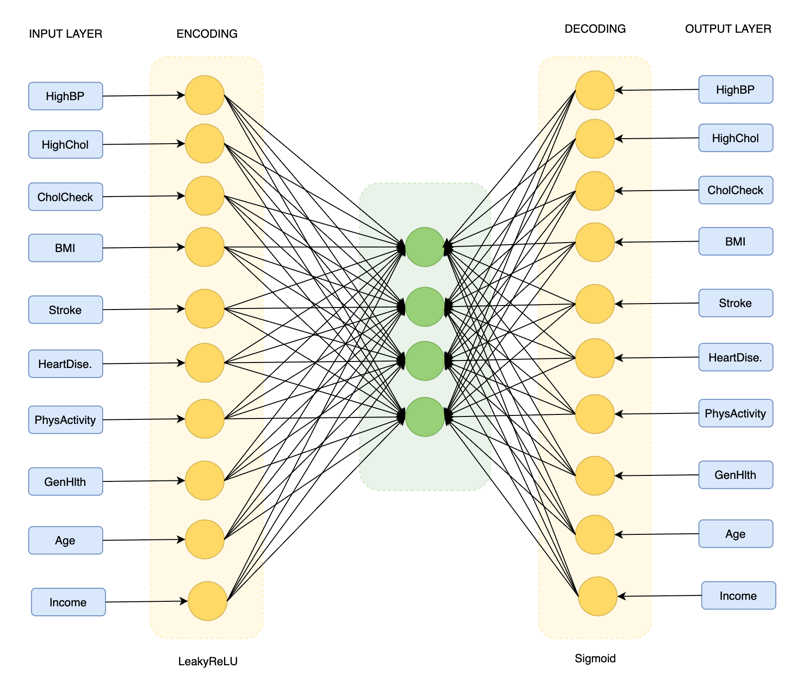
\includegraphics[width=0.7\textwidth]{images/autoencoder.png}
\end{center}
\vspace{0.5cm}

\subsubsection{Finding the best match for the parameters}


\begin{table}[H]
    \centering
    \begin{tabularx}{0.7\textwidth}{
        !{\color{bordergreen}\vrule} m{1.5cm}
        !{\color{bordergreen}\vrule} m{1.5cm}
        !{\color{bordergreen}\vrule} m{1.5cm}
        !{\color{bordergreen}\vrule} m{1.5cm}
        !{\color{bordergreen}\vrule} m{1.5cm}
        !{\color{bordergreen}\vrule} m{1.5cm}
        !{\color{bordergreen}\vrule} m{1.5cm}
        !{\color{bordergreen}\vrule}}
        \hline
        \rowcolor{darkgreen}
        \multicolumn{7}{!{\color{bordergreen}\vrule}c!{\color{bordergreen}\vrule}}{\textbf{\textcolor{white}{}}} \\
        \hline
        \rowcolor{lightgreen}
        \textbf{Model} & \textbf{Activation} & \textbf{Optimizer} & \textbf{Loss} & \textbf{Learning Rate} & \textbf{Accuracy} & \textbf{Recall} \\
        \hline
        Model 1 & ReLU & Adam & MSE & 0.1 & 0.7212 & 0.7212 \\
        \hline
        Model 2 & ReLU & Adam & MSE & 0.3 & 0.7231 & 0.7231 \\
        \hline
        Model 3 & Sigmoid & Adam & Binary CE & 0.1 & 0.5 & 0.5 \\
        \hline
        Model 4 & Sigmoid & Adam & Binary CE & 0.3 & 0.5 & 0.5 \\
        \hline
        Model 5 & ReLU & SGD & MSE & 0.1 & 0.6915 & 0.6915 \\
        \hline
        Model 6 & ReLU & SGD & MSE & 0.3 & 0.7017 & 0.7017 \\
        \hline
        Model 7 & Sigmoid & SGD & Binary CE & 0.1 & -- & -- \\
        \hline
        Model 8 & Sigmoid & SGD & Binary CE & 0.3 & -- & -- \\
        \hline
    \end{tabularx}
    \caption{Model Performance Metrics: Set 1}
    \label{tab:model_performance_set1}
\end{table}








\subsubsection{Implementation}
In order to implement the autoencoder, we will use the \codebox{keras} library. The autoencoder will only function as a feature extractor, for the classification task we will need the {GradientBoostingClassifier} from \codebox{sklearn} library.\\

\noindent The dataset is used the same as for the other algorithms, from the training and testing files.

\vspace{0.5cm}
\lstinputlisting[language=python]{../code/autoencoder/separate_code_for_report/preparation.py}
\vspace{0.5cm}

\noindent Next, the Autoencoder class contains all the logic for the feature extraction task. First the input layer is constructed from keras.layer library. Than encoder is built from the Dense method, also from the keras library, together with the LeakyReLU decoder. The autoencoder is parametrized with the input layer, and two optimization functions are given. Lastly the model is trained with the training set and a batch size of 32. After all the preparations, the model should be trained with the testin set part. The last step will be running the model encoding for the testing set.

\vspace{0.5cm}
\lstinputlisting[language=python]{../code/autoencoder/separate_code_for_report/autoencoder_class.py}
\vspace{0.5cm}

\noindent

\noindent The remaining step will be running the algorithm.
We will first instantiate an encoder from the class we just built, using leaky relu for the first activation function and sigmoid for the second.
As optimizer functions adam and mse are used.
Encoding dim is set to four, for the four attributes to be mapped to, and 50 epochs are used for training.
The output of the encoder is passed to Gradient Boosting Classifer, for the prediction task.
To finish off, we print the confusion matrix, since in our case, as it was also mentioned before, the recall plays a more important role than the accuracy, so this step is unevitable.\\

\vspace{0.5cm}
\lstinputlisting[language=python]{../code/autoencoder/separate_code_for_report/usage.py}
\vspace{0.5cm}
